\documentclass[../sotsu.tex]{subfiles}

\begin{document}


\section{級数}
\label{sec:series}


\subsection{関数の列}

わかりやすくするために,
実数から実数への関数を考える.

\begin{definition}
    \label{dfn:pointwise-convergence}
    関数の列$\sequ{f_n}[n \in \symbb{N}]$が関数$f$に%
    \word{各点収束}[かく|てん|しゅう|そく]%
    \index{かくてんしゆうそく@各点収束}%
    するとは,
    任意の$x \in \symbb{R}$について,
    任意の$\varepsilon > 0$に対し,
    ある$N \in \symbb{N}$が存在して,
    $n > N$なら$\abs{f(x) - f_n (x)} < \varepsilon$となることをいう.
\end{definition}

各点収束の定義は,
「任意の$x \in \symbb{R}$に対し,
$\lim_{n \to \infty} f_n (x) = f(x)$」とかける.

\begin{definition}
    \label{dfn:uniform-convergence}
    関数の列$\sequ{f_n}[n \in \symbb{N}]$が関数$f$に%
    \word{一様収束}[いち|よう|しゅう|そく]%
    \index{いちようしゆうそく@一様収束}%
    するとは,
    任意の$\varepsilon > 0$に対し,
    ある$N \in \symbb{N}$が存在して,
    任意の$x \in \symbb{R}$に対し,
    $n > N$なら$\abs{f(x) - f_n (x)} < \varepsilon$となることをいう.
\end{definition}

2つの定義はよく似ているが,
「任意の$x \in \symbb{R}$」の位置が違う.
$\varepsilon$を固定したとき,
各点収束では$N$が$x$に依存する数$N_{\varepsilon, x}$でよい.
しかし,一様収束では$N$が$x$に依存しない($\varepsilon$のみに依存する)定数$N_\varepsilon$でなくてはならない.


\begin{figure}[tbp]
    \centering
    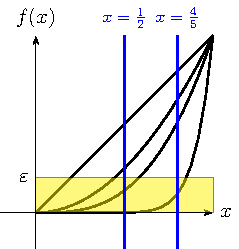
\includegraphics[width=0.4\linewidth]{uniform_convergence_not.pdf}
    \caption{
        $f_n (x) = x^n$のグラフ.
        $n$が大きくなるほど右側のグラフになる.
        $0 < x < 1$で$f_n (x) \to 0$なので,
        グラフは$n \to \infty$で$f(x) < \varepsilon$の領域に収まるはず.
        しかし,左から2番目のグラフだと$x \geq 1/2$でグラフが下側に収まらない.
        $n$を大きくして3番目のグラフにしても,
        $x \geq 4/5$ではグラフが収まらない.
        さらに$n$を大きくして4番目のグラフにしても,
        $x = 4/5$は収まるものの$x \geq 7/8$あたりでやはりグラフがはみ出る.
    }
    \label{fig:uniform-convergence-not}
\end{figure}

\begin{example}
    自然数$n$に対し,関数$f_n$を$f_n (x) \coloneq x^n$($0 \leq x \leq 1$)で定義する(\cref{fig:uniform-convergence-not}).
    $f_n$は$n \to \infty$で
    \begin{equation*}
        f (x) = 
        \begin{cases}
            0  &  (0 \leq x < 1)  \\
            1  &  (x = 1)
        \end{cases}
    \end{equation*}
    に各点収束する.
    しかし,一様収束はしない.
    実際,ある$0 < \varepsilon < 1$を定めたとき,
    $N \in \symbb{N}$をどう取っても,
    $x = \varepsilon^{1/N}$において$x^n > \varepsilon$($n > N$)であるから,
    一様収束の条件を満たさない.
\end{example}


定義から,以下が成り立つ.

\begin{proposition}
    一様収束する関数列は各点収束する.
\end{proposition}






\end{document}